\documentclass[11pt,twoside]{article}
% Shared formatting for all notes in this repository.
% Adapted from the UC Berkeley EECS CS267 lecture-note template:
% https://www.cs.cmu.edu/~ggordon/10725-F12/template.tex
% Personal-note adaptation: boxed title/author/date; ordinary numbering;
% existing natbib citations and mathematical environments are retained.
% Load after \documentclass; compile from the repository root.
\usepackage[T1]{fontenc}
\usepackage[utf8]{inputenc}
\usepackage{amsmath,amsfonts,amssymb,mathrsfs,amsthm}
\usepackage{graphicx,wrapfig}
\usepackage[inline,shortlabels]{enumitem}
\usepackage{centernot}
\usepackage[numbers]{natbib}
\usepackage{adjustbox,booktabs,arydshln}
\usepackage{caption,subcaption}
\usepackage{xcolor,tikz,pifont}
\usetikzlibrary{decorations.pathreplacing,angles,quotes,shapes.geometric,
  arrows.meta,positioning,calc,fit,backgrounds,shadows}
\usepackage[ruled,vlined]{algorithm2e}
\usepackage{xr}
\usepackage{hyperref}
\hypersetup{colorlinks=true,linkcolor=blue,citecolor=blue,urlcolor=blue}

% Berkeley EECS lecture-note page layout and paragraph spacing.
\setlength{\oddsidemargin}{0.25in}
\setlength{\evensidemargin}{-0.25in}
\setlength{\topmargin}{-0.6in}
\setlength{\textwidth}{6.5in}
\setlength{\textheight}{8.5in}
\setlength{\headsep}{0.75in}
\setlength{\parindent}{0in}
\setlength{\parskip}{0.1in}

% A wrapping box accommodates long research-note titles.
\makeatletter
\renewcommand{\maketitle}{%
  \pagestyle{myheadings}%
  \thispagestyle{plain}%
  \begin{center}
    \fbox{%
      \begin{minipage}{\dimexpr\textwidth-2\fboxsep-2\fboxrule\relax}
        \vspace{2mm}
        \textbf{Research Notes}\hfill\@date\par
        \vspace{2mm}
        {\centering\Large\bfseries\@title\par}
        \vspace{2mm}
        {\itshape Author: \@author\par}
        \vspace{2mm}
      \end{minipage}%
    }
  \end{center}
  \markboth{Research Notes}{Research Notes}%
  {\footnotesize\itshape
    Style adapted from the UC Berkeley EECS lecture-note template.\par}
  \vspace{4mm}%
}
\makeatother

\newcommand{\bR}{{\boldsymbol R}}
\newcommand{\bX}{{\boldsymbol X}}
\newcommand{\bY}{{\boldsymbol Y}}
\newcommand{\by}{{\boldsymbol y}}
\newcommand{\bx}{{\boldsymbol x}} 
\newcommand{\bz}{{\boldsymbol z}}
\newcommand{\bZ}{{\boldsymbol Z}}
\newcommand{\bH}{{\boldsymbol H}}
\newcommand{\bb}{{\boldsymbol b}}
\newcommand{\be}{{\boldsymbol e}}
\newcommand{\bbf}{{\boldsymbol f}}
\newcommand{\bg}{{\boldsymbol g}}
\newcommand{\bm}{{\boldsymbol m}}
\newcommand{\bw}{{\boldsymbol w}}
\newcommand{\bW}{{\boldsymbol W}}
\newcommand{\bv}{{\boldsymbol v}}
\newcommand{\bt}{{\boldsymbol t}}
\newcommand{\bA}{{\boldsymbol A}}
\newcommand{\ba}{{\boldsymbol a}}
\newcommand{\bD}{{\boldsymbol D}}
\newcommand{\bE}{{\boldsymbol E}}
\newcommand{\bi}{{\boldsymbol i}}
\newcommand{\bc}{{\boldsymbol c}}
\newcommand{\bC}{{\boldsymbol C}}
\newcommand{\bk}{{\boldsymbol k}}
\newcommand{\bK}{{\boldsymbol K}}
\newcommand{\bP}{{\boldsymbol P}}
\newcommand{\mK}{\mathcal{K}}
\newcommand{\bV}{{\boldsymbol V}}
\newcommand{\bG}{{\boldsymbol G}}
\newcommand{\mG}{\mathcal{G}}
\newcommand{\mH}{\mathcal{H}}
\newcommand{\mE}{\mathbb{E}}
\newcommand{\mX}{\mathcal{X}}
\newcommand{\mM}{\mathcal{M}}
\newcommand{\bU}{{\boldsymbol U}}
\newcommand{\bu}{{\boldsymbol u}}
\newcommand{\bI}{{\boldsymbol I}}
\newcommand{\bJ}{{\boldsymbol J}}
\newcommand{\bs}{{\boldsymbol s}}

\newcommand{\bxi}{{\boldsymbol \xi}}
\newcommand{\balpha}{{\boldsymbol \alpha}}
\newcommand{\bbeta}{{\boldsymbol \beta}}
\newcommand{\bgamma}{{\boldsymbol \gamma}}
\newcommand{\btheta}{{\boldsymbol \theta}}
\newcommand{\bTheta}{{\boldsymbol \Theta}}
\newcommand{\bvartheta}{{\boldsymbol \vartheta}}
\newcommand{\bepsilon}{{\boldsymbol \epsilon}}
\newcommand{\bvarepsilon}{{\boldsymbol \varepsilon}}
\newcommand{\bomega}{{\boldsymbol \omega}}
\newcommand{\bmu}{{\boldsymbol \mu}}
\newcommand{\bSigma}{{\boldsymbol \Sigma}}

\newcommand{\corr}{\mbox{Corr}}
\newcommand{\var}{{\mbox{Var}}}
\newcommand{\Var}{{\mbox{Var}}}
\newcommand{\cov}{{\mbox{Cov}}}
\newcommand{\diag}{{\mbox{diag}}}
\newcommand{\bUmis}{{\boldsymbol U}_{{\rm mis}}}
\newcommand{\bYmis}{{\boldsymbol Y}_{{\rm mis}}}
\newcommand{\bYobs}{{\boldsymbol Y}_{{\rm obs}}}
\newcommand{\tbXmis}{{\tilde{\boldsymbol X}}_{{\rm  mis}}}
\newcommand{\tbxmis}{{\tilde{\boldsymbol x}}_{{\rm  mis}}}
\newcommand{\bXmis}{{\boldsymbol X}_{{\rm mis}}}
\newcommand{\bXobs}{{\boldsymbol X}_{{\rm obs}}}
\newcommand{\bZmis}{{\boldsymbol Z}_{{\rm mis}}}
\newcommand{\bZobs}{{\boldsymbol Z}_{{\rm obs}}}
\newcommand{\tXmis}{{\tilde{X}}_{{\rm  mis}}}
\newcommand{\txmis}{{\tilde{x}}_{{\rm  mis}}}
\newcommand{\Xmis}{X_{{\rm  mis}}}
\newcommand{\Xobs}{X_{{\rm  obs}}}
\newcommand{\bymis}{{\boldsymbol y}_{{\rm  mis}}}
\newcommand{\byobs}{{\boldsymbol y}_{{\rm  obs}}}
\newcommand{\ymis}{y_{{\rm  mis}}}
\newcommand{\yobs}{y_{{\rm  obs}}}

\newcommand{\JRSSB}{Journal of the Royal Statistical Society: Series B}
\newcommand{\indep}{\rotatebox[origin=c]{90}{$\models$}}
\newcommand{\red}{\textcolor{red}}
\newcommand{\blue}{\textcolor{blue}}
\newcommand{\notetodo}[1]{\textcolor{blue}{[TODO: #1]}}

% Preserve the existing independent, section-based theorem counters.
\newtheorem{theorem}{Theorem}[section]
\newtheorem{lemma}{Lemma}[section]
\newtheorem{corollary}{Corollary}[section]
\newtheorem{formula}{Formula}[section]
\newtheorem{proposition}{Proposition}[section]
\theoremstyle{definition}
\newtheorem{definition}{Definition}[section]
\newtheorem{example}{Example}[section]
\newtheorem{assumption}{Assumption}
\theoremstyle{remark}
\newtheorem{remark}{Remark}

% Journal abbreviations used by the existing bibliography.
\def\AJE{American Journal of Epidemiology}
\def\ANNALS{Annals of Statistics}
\def\BIOK{Biometrika}
\def\BMCS{Biometrics}
\def\STATMED{Statistics in Medicine}
\def\STATSCI{Statistical Science}
\def\JSPI{Journal of Statistical Planning \& Inference}
\def\JRSSB{Journal of the Royal Statistical Society, Series B}
\def\COMMS{Communications in Statistics, Series A}
\def\JQT{Journal of Quality Technology}
\def\TECH{Technometrics}
\def\JASA{Journal of the American Statistical Association}
\def\CSDA{Computational Statistics \& Data Analysis}
\def\JCGS{Journal of Computational and Graphical Statistics}
\def\JCB{Journal of Computational Biology}
\def\BIOINF{Bioinformatics}
\def\JAMA{Journal of the American Medical Association}
\def\JNUTR{Journal of Nutrition}
\def\LETTERS{Letters in Probability and Statistics}
\def\JABES{Journal of Agricultural, Biological and Environmental Statistics}
\def\SCAN{Scandinavian Journal of Statistics}
\def\PNAS{Proceedings of the National Academy of Sciences USA}
\def\JMLR{Journal of Machine Learning Research}
\def\JSCS{Journal of Statistical Computation and Simulation}

\clubpenalty=10000
\widowpenalty=10000

\title{Causal Inference Basics}
\author{Wen-Hung Wang}
\date{\today}

% Transcribed from the two-page handwritten note "Causal basics.pdf".
% The handwritten exogenous-error glyphs are normalized to e_{yi} in
% both the factual and potential-outcome equations below.

\begin{document}
\maketitle
\textbf{Abstract.} This note discusses some basic concepts used is my causal inference project. Specifically, it does not discuss topics on causal graphs such as structural learning. We focus on inference given a DAG, with a focus on missing confounder problems. Several methodologies tackling this problem are briefly introduced. 

\tableofcontents
\bigskip
\section{Introduction}
Identifying causality has been of interest in scientific field for decades. However, randomized trials, which is the gold standard in causal inference, might not be used due to various reasons such as ethical issues, high costs, etc. Observational data, on the other hand, is easier to obtain but lack some desired control in order to make causal statements. For example, the existence of unmeasured confounders relates treatments and outcomes, violating the exchangeability condition. Thus, making causal claims from observational data is at the heart of causal inference. 

Here are three types of randomized designs
\begin{itemize}
    \item Completely randomized design: $n_1$ out of $n$ objects randomly assigned to the treatment.
    \item Bernoulli design: for each individual, assignment treatment according a Bernoulli($p$) random variable.
    \item Matched pair design: match individuals into pairs and randomly assign treatment among them.
\end{itemize}


\section{Potential Outcomes and Causal Estimands}
\label{sec:potential-outcomes}

Let $Y_i(a)$ be the \emph{potential outcome} of individual $i$ under treatment level $a$.
\begin{itemize}
    \item Binary treatment: The average treatment effect (ATE) is
    \begin{equation}
    \label{eq:ate}
        \operatorname{ATE} = E\big[Y(1)-Y(0)\big].
    \end{equation}
    \item Continuous treatment: The \emph{dose-response function} is
    \begin{equation}
    \label{eq:dose-response}
        \mu(a) = E\big[Y(a)\big].
    \end{equation}
\end{itemize}

\begin{remark}
    Individual treatment effect (ITE) is defined as $Y_i(a)-Y_i(a')$. 
\end{remark}

A fundamental challenge in causal inference is the counterfactual (the \emph{what if}, missing data problem). For each individual, we only observe the potential outcome corresponding to the intervention actually received; the alternative intervention remains unobserved.


\subsection{Factual and Potential Outcomes in an SCM}

Suppose the factual outcome is generated by the structural equation
\begin{equation}
\label{eq:factual-outcome}
    y_i = \mu_3(a_i,z_i,\theta_3) + \sigma_3 e_{yi}.
\end{equation}
Under the structural causal model (SCM), setting the treatment to $a$
 gives the potential outcome
\begin{equation}
\label{eq:potential-outcome}
    Y_i(a) = \mu_3(a,z_i,\theta_3) + \sigma_3 e_{yi}.
\end{equation}
The same individual-level exogenous error is held fixed under the
 intervention. Thus,
\begin{equation}
\label{eq:consistency}
    \underbrace{y_i}_{\textcolor{red}{\text{observation}}}
    = \underbrace{Y_i(a_i)}_{\textcolor{blue}{\text{causal quantity}}},
\end{equation}
which satisfies \emph{consistency}.

\begin{remark}[Factual versus causal quantities]
$Y$ is the factual outcome, an observational (non-causal) quantity.
$Y(a)$ is a potential outcome, a causal quantity. In $Y(a)$, the
 treatment level $a$ is fixed.
\end{remark}

The central question is:
\begin{quote}
\textcolor{red}{How can we express a causal estimand as a functional of
 the observational distribution?}
\end{quote}
That is, how can we make causal claims from observational data?

\section{Linking Causal Estimands to Observational Data: Adjustment Formula and Inverse Propensity Weighting}
\label{sec:identification}

To estimate causal estimand from observational data, the so-called $g-$formula or adjustment formula is used. Assume the following conditions.
\begin{assumption}[Consistency]
The observed outcome agrees with the potential outcome at the
 observed treatment level: $Y=Y(A)$, or, equivalently, \(Y=AY(1)+(1-A)Y(0)\) for binary treatments.
\end{assumption}

\begin{assumption}[Conditional ignorability/exchangeability]
For each treatment level $a$ of interest,
\begin{equation}
\label{eq:ignorability}
    Y(a) \mathrel{\indep} A \mid Z.
\end{equation}
Note that this is weak ignorability \cite{Hirano2004}. Strong ignorability \cite{rosenbaum1983central} says $ \{Y(a), a \in \mathcal{A}\} \mathrel{\indep} A \mid Z.$
\end{assumption}

\begin{assumption}[Positivity or overlap]
For binary treatment,
\begin{equation}
\label{eq:binary-positivity}
    0 < P(A=1\mid Z=z) < 1.
\end{equation}
For continuous treatment, the corresponding density condition is
\begin{equation}
\label{eq:continuous-positivity}
    f_{A\mid Z}(a\mid z)>0
\end{equation}
for the treatment levels of interest and almost every $z$ in the
 target population.
\end{assumption}

Under these assumptions, there are two methods to identify average effects:
\begin{itemize}
    \item $g-$formula/ standardization: using outcome regression $E[Y|Z,A]$.
    \item Inverse propensity weighting: using propensity score, $P(A=1|Z)$.
\end{itemize}

\begin{remark}
    Crucially, observational data often fails to satisfy conditional ignorability due to unmeasured confounders. Therefore, in practice, practitioners have to use domain knowledge to include as many as confounders. However, including too many variables is problematic too.
\end{remark}

\subsection{$g-$formula/ standardization} 
Under these assumptions, 
\begin{align}
\label{eq:adjustment-derivation}
    \underbrace{E\big[Y(a)\big]}_{\text{causal}}
    &= E_Z\!\left[E\big[Y(a)\mid Z\big]\right] \notag\\
    &= E_Z\!\left[E\big[Y(a)\mid Z,A=a\big]\right] \notag\\
    &= E_Z\!\left[E\big[Y\mid Z,A=a\big]\right] \notag\\
    &= \int \underbrace{E\big[Y\mid Z=z,A=a\big]}_{\text{observational}}\,dF_Z(z).
\end{align}
The first equality uses iterated expectation, the second uses
 conditional ignorability, and the third uses consistency.
The conditional mean $E[Y\mid Z=z,A=a]$ is an observational quantity.

$Z$ is the \emph{adjustment set}. The resulting expression,
\begin{equation}
\label{eq:g-formula}
    \boxed{\mu(a)=\int E\big[Y\mid A=a,Z=z\big]\,dF_Z(z)},
\end{equation}
is called the \emph{adjustment formula} or \emph{$g$-formula}.

\begin{remark}[Scope of the research]
In our research, we do not address causal discovery or adjustment-set
 selection. The causal directed acyclic graph (DAG) is already given.
Causal graphs can be used to find adjustment sets, for example through
 the \emph{back-door criterion.}
\end{remark}

\subsection{Inverse propensity weighting}
The motivation of propensity score is to study causality using observational data, i.e., identify causal effect. The basic idea behind IPW is to link association to causality through reweighting outcomes. We first consider a discrete confounder example in which $Z$ is discrete.
\[
E[Y(a)] = \underbrace{\sum_z E[Y|A=a,Z=z]\textcolor{blue}{P(Z=z)}}_{g-\text{formula}} 
\]
while association quantity is, by iterated expectation 
\[
E[Y|A=a] = E[E[Y|A=a,Z]|A=1] = \sum_z E[Y|A=a,Z]\textcolor{blue}{P(Z=z|A=a)}.
\]
So the question becomes can we find a $f(a,z)$ such that 
\[
\sum_z E[Y|A=a,Z=z]\textcolor{blue}{P(Z=z|A=a)}\textcolor{red}{f(z,a)} = \underbrace{\sum_z E[Y|A=a,Z=z]\textcolor{blue}{P(Z=z)}}_{g-\text{formula}}.
\]
Thus taking 
\[
\boxed{
f(z,a) = \frac{P(Z=z)}{P(Z=z|A=a)} = \frac{P(A=a)}{P(A=a|Z=z)}}
\]
gives the desired result. It can be shown that, under the above assumptions
\[
E[Y(a)] = E\left[Y \frac{P(A=a)}{P(A=a|Z)}|A=a\right] = E\left[Y \frac{I(A=a)}{P(A=a|Z)}\right], 
\]
which consists only observed data.
\begin{remark}
    This analysis suggests that the imbalance problem $P(Z=z) \neq P(Z=z|A=a)$ is the main cause for this fact, i.e., covariate (confounder) distribution in different treatment groups is not the same. 
\end{remark}


Let's consider a binary treatment first. 
\begin{definition}[Propensity Score]
    The propensity score \cite{rosenbaum1983central} is defined as 
    \[
    e(z) = P(A=1|Z=z),
    \]
    which can be estimated by logistic regression.
\end{definition}

\emph{Inverse Propensity Weighting (IPW)} estimates the ATE using
\[
\boxed{
\widehat{\tau}_{\mathrm{IPW}}
=
\frac1n\sum_{i=1}^n
\left[
\frac{A_iY_i}{\widehat e(Z_i)}
-
\frac{(1-A_i)Y_i}{1-\widehat e(Z_i)}
\right],}
\]
This is called Horvitz–Thompson estimator \cite{Horvitz01121952}. To see why we use this estimator, we compute, assuming consistency, conditional ignorability, and positivity
\begin{align*}
    E\left[\frac{AY}{ e(Z)}\right] &= E_Z\left\{E\left[\frac{AY}{e(Z)}\big|Z\right]\right\} \\
    &= E_Z\left\{E\left[\frac{AY(1)}{e(Z)}\big|Z\right]\right\} \\
    &= E_Z\left\{E\left[A\big|Z\right]E\left[\frac{Y(1)}{e(Z)}\big|Z\right]\right\} \\
    & = E_Z\left\{\frac{P(A=1|Z)}{e(Z)}E\left[{Y(1)}\big|Z\right]\right\} = E[Y(1)].
\end{align*}
Similarly, we can show that $E\left[\frac{(1-A)Y}{1-e(Z)}\right]=E[Y(0)]$.

\section{Confounding: Correlation versus Causation}
\label{sec:confounding}

Suppose that $Z$ is a confounder. Without adjustment, correlation
 need not represent causation. Consider the causal graph
\begin{center}
\begin{tikzpicture}[>=Stealth,
    every node/.style={circle,draw,minimum size=8mm,inner sep=1pt}]
    \node (Z) at (0,1.5) {$Z$};
    \node (A) at (-1.3,0) {$A$};
    \node (Y) at (1.3,0) {$Y$};
    \draw[->] (Z) -- (A);
    \draw[->] (Z) -- (Y);
    \draw[->] (A) -- (Y);
\end{tikzpicture}
\end{center}

\paragraph{A Linear Gaussian Example}
Consider
\begin{align}
\label{eq:gaussian-model}
    Z,e_a,e_y,e_1,e_2 &\sim N(0,1), \notag\\
    A &= Z+e_a, \notag\\
    Y &= \tau A+\beta Z+\sigma_y e_y, \notag\\
    X_1 &= Z+s e_1, \qquad X_2=Z+s e_2.
\end{align}
The covariance calculation below takes the exogenous variables
 $Z,e_a,e_y,e_1,e_2$ to be mutually independent.
% Independence is implicit in the handwritten covariance calculation.

Regressing $Y$ on $A$ alone, or minimizing $E[(Y-tA)^2]$ over $t$,
 gives the population regression coefficient
\begin{align}
\label{eq:confounding-bias}
    \tau_{\mathrm{naive}}
    &= \frac{\cov(Y,A)}{\var(A)} \notag\\
    &= \frac{\cov(\tau A+\beta Z+\sigma_y e_y,A)}{\var(A)} \notag\\
    &= \frac{\tau\var(A)+\beta\cov(A,Z)}{\var(A)} \notag\\
    &= \tau+\beta\frac{\cov(A,Z)}{\var(A)} \notag\\
    &= \tau+\underbrace{\frac{1}{2}\beta}_{\textcolor{red}{\text{confounding bias}}}.
\end{align}
Here $\var(A)=2$ and $\cov(A,Z)=1$. Consequently,
\begin{equation}
\label{eq:observational-vs-causal}
    \underbrace{E[Y\mid A=a]=\left(\tau+\frac{1}{2}\beta\right)a}
      _{\text{observational mean}}
    \qquad\text{versus}\qquad
    \underbrace{E[Y(a)]=\tau a}_{\text{causal mean}}.
\end{equation}
Therefore, we need the $g$-formula and adjustment for $Z$. To see this, consider model \eqref{eq:observational-vs-causal} where $Z$ is assumed observable here; then regressing $Y$ on \emph{both} $A$ and $Z$ gives an estimate of $E[Y|Z=z,A=a]$ in $g-$formula \eqref{eq:g-formula}, denoted as $\hat{m}(a, Z_i)=\hat{\tau}a + \hat{\beta}Z_i$. The estimated dose-response function becomes
\[
\hat{\mu}(a) = \widehat{E[Y(a)]} = \frac{1}{n}\sum_{i=1}^n\hat{m}(a, Z_i).
\]
One may estimate $\mu(a)-\mu(a')$ by 
\[
\frac{1}{n}\sum_{i=1}^n\hat{m}(a, Z_i) - \frac{1}{n}\sum_{i=1}^n\hat{m}(a', Z_i) = \hat{\tau}(a-a')
\]
under the constant $\tau$ assumption.

\section{The Problem of Missing Confounders}
\label{sec:missing-confounders}

Recall the adjustment formula:
\begin{align}
\label{eq:missing-confounder-formula}
    E[Y(a)]
    &= E_Z\!\left[E[Y\mid A=a,Z]\right] \notag\\
    &= \int
       \underbrace{E[Y\mid A=a,Z=z]}_{\text{outcome regression}}
       \underbrace{dF_Z(z)}_{\text{confounder distribution}}.
\end{align}
\textcolor{red}{Both components require information about $Z$.}

If $Z$ is missing, we ask whether $\tau$ can be identified from
\[
    (Y,A)
    \qquad\text{or}\qquad
    (Y,A,\underbrace{X}_{\text{proxy}}).
\]
In the example above, $X=(X_1,X_2)$ consists of noisy proxies for $Z$.
Some related works study identification conditions for such models.

\clearpage
\bibliography{ref}
\bibliographystyle{abbrv}

\end{document}
